\chapter{Architecture of a Quantum Computer}
\label{sec:arch}
Although the challenges of building a fault-tolerant qubit have by no means been overcome, the field is rapidly reaching the point where
it is possible to start running algorithms on quantum computers. While algorithms such as Shor's algorithm for prime factorization
requires a large number of qubits with arbitrarily long lifetimes~\cite{Beauregard:2003,6657074}, other algorithms may
be able to achieve a quantum speedup with a limited number of noisy qubits. Algorithms and systems operating in this regime are
said to be in the Noisy Intermediate-Scale Quantum (NISQ) regime~\cite{Preskill2018quantumcomputingin}, a term coined by John Preskill
to distinguish between a full-scale quantum computer with a large number of error corrected qubits, and a machine containing as few
as 10s of noisy, imperfect qubits that we may realize in the coming decade. In the near term, the race is on to achieve \textbf{quantum supremacy},
a calculation on a quantum computer whose simulation on a classical computer is intractable. The expectation is that this milestone will
be beaten in the coming years, with a system of approximately 50 noisy qubits~\cite{s41567-018-0124-x}. Based on the current state of the field
this will likely occur using superconducting transmon-like qubits solving a model problem such as Boson sampling~\cite{Aaronson:2011}. While such a
result would certainly be groundbreaking, the more interesting result would be a demonstration of \textbf{quantum advantage}, an algorithm whose simulation on a
classical computer is intractable, but one which also solves a useful problem. While Boson sampling certainly seems to be a classically hard problem,
the solution it provides does not seem to be one that has many practical implications. In the near term, our best bet for achieving a useful result
seems to be using the Variational Quantum Eigensolver algorithm \cite{ncomms5213}, which, as we alluded to in the introduction of Chapter~\ref{sec:quest}, would allow us
to model molecules that we could not on a classical computer, with a small number (100s) of imperfect qubits~\cite{PhysRevA.92.042303}.
To date, several experimental realizations of this algorithm have been published~\cite{nature23879,PhysRevX.8.011021,10.1038/s41586-019-1040-7},
although none have yet simulated a molecule that is classically intractable~\cite{Reiher7555}.

\section{Designing an Architecture}
\label{sec:archdesign}
Given the rapid progression of the field, the questions surrounding architecting a quantum computer have been gaining increasing attention,
particularly as the number of qubits grows beyond the limits that we might control with an ad-hoc architecture that a single graduate student might construct.
The challenge for experimentalists continues to come down to building scalable building blocks, which balance the need for experimental
flexibility surrounding qubits whose designs and control requirements remain in flux, but whose footprint does not explode for larger numbers
of physical qubits. Thankfully, there is substantial overlap in the requirements for control and readout between qubit implementations
(at least within the realm of superconductor and semiconductor based qubits), which allows us to design architectures for hypothetical
quantum machines. Let's therefore enumerate a few of the key requirements for a control and readout architecture for solid-state qubits:
\begin{itemize}
  \item \textbf{Cryogenic operation}: Solid-state qubits must be operated in cryogenic environments, stemming from the requirement that the thermal energy should be well below the level spacing of energy levels in the qubit, as well as the need for superconducting elements in some designs. Any control and readout architecture must, therefore, be low power, and avoid carrying thermal energy or noise down to the qubit device.
  \item \textbf{Control fidelity}: In order to reach the fault-tolerance threshold, fidelities of individual qubits must exceed $99\%$, and should ideally be well above the $(1 - 10^{-5})$ level to avoid prohibitive error correction requirements~\cite{6657074}. Depending on the rotation rate and decoherence rates of individual qubits, control lines must have bandwidths of several 10's of \si{\giga\hertz}, as well as being high density while maintaining low crosstalk.
  \item \textbf{Readout fidelity}: Readout of qubits brings unique challenges, requiring low probe powers in order to avoid disturbing the state while it is being measured, and limited measurement time due to decoherence. In addition, QEC in general requires the continued measurement of ancilla qubits while nearby qubits are operational, leading to stringent crosstalk requirements. In order to obtain sufficient signal-to-noise ratio, cryogenic amplification is generally required, which in turn limits scalable designs to a small number of parallel readout lines. As such, some form of multiplexing, either frequency-domain or time-domain, is necessary for readout.
  \item \textbf{Space}: This requirement is particularly difficult to accomplish as it occurs over three orders of magnitude over the scale of the chip, the cryostat and at room temperature. Each of these are discussed in detail below, but we state the problem briefly here. On a chip scale, dense control lines must be fit into an area set by the distance over which we can achieve coupling between qubits, setting micron-scale limits on on-chip structures. On a cryostat level, the need to operate at \si{\milli\kelvin} places centimeter-scale limits on cryogenic components. Finally at room temperature, phase matching of control pulses and the need for active feedback places limits on the size of the instrumentation used to control individual qubits.
\end{itemize}

\afterpage{
  \clearpage
  \thispagestyle{empty}
  \begin{landscape}
  \begin{table}
    \centering
    \def\arraystretch{1.5}
    \begin{tabular}{lllllll}
    \toprule
    \multicolumn{3}{l}{} & \shortstack{CryoCMOS Architecture\\(Section~\ref{sec:gooseberry})} & \shortstack{Prime-Lines Architecture\\(Section~\ref{sec:primelines})} & \shortstack{Frequency\\Multiplexed~\cite{doi:10.1063/1.4868107}} & \multicolumn{1}{c}{Na\"ive} \\
    \midrule
    \multirow{5}{*}{Room Temp}  & \multirow{2}{*}{Power} & $P_{C,RT}$    & $\SI{100}{\watt}$ & $M\times\SI{1000}{\watt}$ &$N\times\SI{1000}{\watt}$ &$N\times\SI{1000}{\watt}$\\
                                &                        & $P_{R,RT}$    & $\SI{100}{\watt}$ & $N\times\SI{100}{\watt}$ & $N\times\SI{100}{\watt}$ & $N\times\SI{100}{\watt}$\\\cline{2-7}
                                & \multirow{3}{*}{Lines} & $L_{DC,C,RT}$ & 3                         & $N$                      & $N$ & $N$                 \\
                                &                        & $L_{RF,C,RT}$ & 3                         & M                        & $N$ & $N$                 \\
                                &                        & $L_{RF,R,RT}$ & 2                         & 2                        & 2   & $N$                 \\\hline
    \multirow{5}{*}{4K} & \multirow{2}{*}{Power} & $P_{C,4K}$    & $\SI{1}{\watt}$        &$\SI{1}{\watt} + M\times\SI{100}{\micro\watt}$        & $N\times\SI{100}{\micro\watt}$   & $N\times\SI{100}{\micro\watt}$                   \\
                        &                        & $P_{R,4K}$    & $\SI{50}{\milli\watt}$ &$\SI{50}{\milli\watt}$ & $\SI{50}{\milli\watt}$ & $N\times\SI{50}{\milli\watt}$\\\cline{2-7}
                        & \multirow{3}{*}{Lines} & $N_{DC,C,4K}$ & 3                         & $N$                      & $N$ & $N$                 \\
                        &                        & $L_{RF,C,4K}$ & 3                         & $M$                      & $N$ & $N$                 \\
                        &                        & $L_{RF,R,4K}$ & 2                         & 2                        & 2   & $N$                 \\\hline
    \multirow{4}{*}{mK} & \multirow{2}{*}{Power} & $P_{C,mK}$ & $N\times\SI{6}{\pico\watt} + \SI{34}{\micro\watt}$ & $ (N+M)\times\SI{1}{\micro\watt}$ & $N\times\SI{1}{\micro\watt}$   & $N\times\SI{1}{\micro\watt}$                   \\
                        &                        & $P_{R,mK}$ & \SI{40}{\nano\watt}     & \SI{40}{\nano\watt}           &\SI{40}{\nano\watt}   & $N\times\SI{40}{\nano\watt}$ \\\cline{2-7}
                        & \multirow{2}{*}{Lines} & $L_{C,mK}$ & $N$                     & $N$                           & $N$ & $N$                 \\
                        &                        & $L_{R,mK}$ & $N$                     & $N$                           & $N$ & $N$                 \\
    \bottomrule
    \end{tabular}
    \caption[Approximate power and wiring requirements for a QC]{Order of magnitude power $P$ and wiring $L$ requirements for the CryoCMOS architecture, the Prime-Lines architecture, frequency multiplexed readout and a Na\"ive architecture. The number of lines is split between high-bandwidth coaxial lines (rf) and low-bandwidth (dc) lines. In each case, we trade off the complexity in the setup to reduce the wiring required down the fridge. The power consumption and number of lines is given in terms of the number of qubits $N$, and in the case of the Prime-Lines architecture, the number of pulse shapes $M$. Power consumption for control lines is calculated assuming a \SI{1}{\milli\volt} pulse at the qubit through a \SI{20}{\decibel} attenuator at the \SI{4}{\kelvin} and mK stage. For the CryoCMOS architecture, a pulse frequency of \SI{10}{\mega\hertz} was used. Readout power is calculated assuming a Caltech-style HEMP amplifier at the 4K stage, and utilizing rf-reflectometry techniques for readout (see Sec.~\ref{sec:readout}). With a \SI{-90}{\decibel} readout power,
    dissipation is dominated by passive thermal conduction up to $\sim 1000$ simultaneous channels.}
    \label{tab:arch}
  \end{table}
\end{landscape}
}

In general, qubit architectures for solid-state qubits can be classified into two categories (control and readout) at three different temperature stages
(room temperature (RT), four Kelvin (4K) and milli-Kelvin (mK)), as shown in Fig.~\ref{fig:genarch}. An
architecture is characterized by the number of rf and dc lines that run between temperature stages $L$, and a power consumption at each stage $P$, divided between the control
and readout block. Two architectures are presented in this thesis, which trade off complexity and reduced experimental flexibility for reduced wiring and power consumption
at different stages of the cryostat. The CryoCMOS architecture, presented in Sec.~\ref{sec:gooseberry} utilizes a CMOS based switching matrix at millikelvin temperatures that is
bonded directly to the qubit chip in order to minimize the power dissipated in parasitic capacitance. The Prime-Lines architecture, presented in Sec.~\ref{sec:primelines}
utilizes a cryogenic switching matrix near the qubit to minimize the number of high-frequency coaxial lines required to control qubits. Order of magnitude estimates
for the number of control lines and the power consumption for each architecture is given in Table~\ref{tab:arch}, characterized by a number of qubits $N$,
and in the case of the prime-lines architecture, the number of control pulse-shapes $M$, where in general $M \ll N$. The sources of power dissipated for each of these architectures
will be elucidated over the course of the remainder of the section. I will however draw the readers attention to the fact that even for passive, high-bandwidth wiring, there is a
power cost associated with bringing these lines down~\cite{Krinner2019}, a topic I will explore in detail in Sec.~\ref{sec:control}.

\begin{figure}
  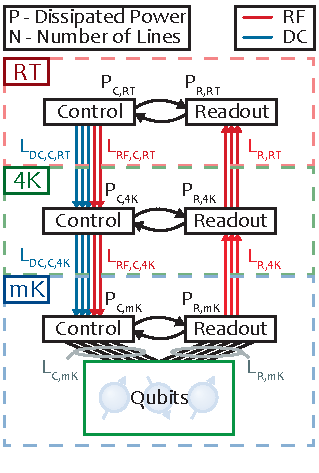
\includegraphics[width=0.5\linewidth]{genarch}
  \caption[Generalized quantum computing architecture]
  {\label{fig:genarch}A generalized qubit architecture, broken into control and readout stages at each temperature stage of a cryostat. The architecture is characterized by number of lines which run between each stage, for example $L_{RF,C,RT}$ for the number of coaxial control lines running from room temperature to the \SI{4}{\kelvin} stage of the cryostat, which will vary depending on the choice of a given architecture. In addition, each stage will dissipate a certain amount of power, for example $P_{R,4K}$ being the power dissipated at \SI{4}{\kelvin} by the readout stage, caused either by active logic, such as an FPGA, amplifiers or off-the-shelf instrumentation, or by passive dissipation, for example due to attenuators.}
\end{figure}

In the remainder of this section, I will quickly review the challenges for control and readout for a large-scale quantum computer, which very much remains
an open question in the field. As we move through the following sections, the sources of many of the numbers in Table~\ref{tab:arch} should become clear
as well as our vision for solving some of these problems. In general, I will progress from the qubit plane up to room temperature control, however this
structure is by no means strict.

\subsection{Control Plane}
\label{sec:control}
A popular refrain for proponents of semiconductor-based qubits is to point to the maturity and flexibility of modern semiconductor processing as an argument
for the scalability of qubits based on similar processes. While it is undoubtedly true that the miniaturization of transistors has translated into an ability
to fabricate finer devices, the scalability of quantum computers based on such an argument is by no means clear. The problem, and indeed the main differentiator
between a qubit and a transistor, it that while a transistor has the ability to drive other transistors, a qubit has no similar ability. All control of a qubit,
to initialize and to drive single and two qubit rotations, must come from outside. This unfortunate fact is captured in Rent's rule, which relates the number of
external terminals (or pins) $T$ of an IC, to the number of internal components (or transistors) $g$:
\begin{equation}
  T = tg^p
  \label{eq:rent}
\end{equation}
where $t$ and $p$ are constants of the system. For an integrated circuit, the value of $p$ generally ranges from 0.5 to 0.8~\cite{5388820}, however for a quantum
circuit, it is reasonably simple to see that this exponent must be 1! Each qubit must be driven by some number $t$ gates, with no qubit able to drive another
qubit without some external control.

The above statement captures the primary difficulty that we will run into when designing qubit chips. While classical ICs can rely on some fan-out to minimize
the number of inputs required, the design of a quantum chip must be able to supply high density wiring with high bandwidth and low cross-talk. In addition,
classical CMOS processes usually have only a few layers of high-density interconnects, used only for short-range connections~\cite{5424258}, while qubit
architectures generally require several layers of high-density interconnects over the length of an entire chip~\cite{s41467-017-01905-6}. The question then is
what sets the maximum pitch of a qubit on a chip, as this gives us the density of control lines that must be achieved. Then, given that pitch, how many lines could
we bring in to such a device, given a 1D or a 2D grid of qubits?

The answer to the first question, the pitch of qubit devices, will be set by the length scale over which coupling can be achieved. For spin qubit devices based only
on direct exchange for example, the pitch of qubits will be roughly the size of the qubit itself, as coupling only occurs when electrons can directly tunnel between
neighbouring devices~\cite{PhysRevB.86.085423}. Work presented in this thesis uses elongated many-electron quantum dots to increase this to the micron-scale in
Section~\ref{sec:5dot}, an approach which will likely be applicable Majorana devices that use quantum dots as couplers~\cite{PhysRevB.95.235305}. Finally, long
distance coupling of spins via superconducting resonators~\cite{PhysRevB.97.235409} has recently been demonstrated~\cite{2019arXiv190500776B}, enabling coupling
over \si{\milli\meter} length scales.

The next question is how many lines we can bring to a device. In a 1D array of qubits, that is for a single line of qubits, the answer is limited only by the
physical size of the chip, and the size of pads (bond pads or bump pads) that we are able to make contact to. For example, a singlet-triplet qubit which requires
10 control lines, and pads of pitch $100\times100\si{\micro\meter}$ will require a chip with a \SI{0.01}{\square\milli\meter} area, assuming of course that we are
able to make contact in 3D (i.e. overlapping bonds). In the case that we are only able to make contact in 2D, a chip of size $400\times400\si{\micro\meter}$ at a
minimum is required to break pads out to the edge of a device.

The situation is more difficult to evaluate in a 2D array. Firstly, a 2D array is not possible on
a single planar grid, as control lines for inner qubits must be broken out. Therefore a sufficient distance between qubits must be possible to allow control lines
to be brought in from upper layers. To allow fan-out of a dense grid leads to a problem very similar to that of routing a ball-grid array (BGA) package. There will
be a relationship between number of layers, track pitch and via (inter-layer contact) pitch, which will set a hard density limit on qubit devices. Therefore
increasing the pitch of qubit devices via long distance coupling may be necessary when moving to 2D grids. Furthermore, the design of qubit layouts allowing
realistic wiring schemes will continue to be crucial moving forwards~\cite{10.1038/s41534-018-0074-2}. Finally, I point to the potential for multiplexing the
control of many qubits onto single control lines, which may allow the definition of a quantum analog to Rent's rule~\cite{FRANKE20191} (Equation~\ref{eq:rent}).
Whether such an architecture is truly scalable remains an open question at this time.

On a single qubit chip it seems difficult to get around the problem of breaking all control lines out in order to allow qubit control. Alluding
back to our generalized qubit architecture in Fig.~\ref{fig:genarch}, it should in general be possible to reduce the number of lines running between the 4K stage
and the control plane at mK. To understand the techniques for doing so, it is useful to separate control pulses into three general forms: microwave excitations,
fast pulses and static confinement. The first two of these require high bandwidth rf wiring, while the latter requires only low bandwidth dc wiring. By the use of
CryoCMOS switches, as detailed in Section~\ref{sec:gooseberry}, it is possible to multiplex a single dc control line to several gates, effectively locking
a voltage onto those gates. Such switches do not dissipate power except when toggled, leading to extremely low power consumption. Similarly, fast pulses may similarly
be generated, again, as detailed in Section~\ref{sec:gooseberry}, minimizing the parasitic capacitance and hence power dissipation, given by $P_\textrm{diss} = CV^2f$,
caused by the length of control lines. Note that in the limit where pulses are generated next to the qubit device we no longer use require the use of a matched transmission
line, allowing calculation of dissipation using this formula. This in turn leads to the low power consumption of the CryoCMOS architecture in Table~\ref{tab:arch}.
The availability of CMOS at low temperature also gives us a possible solution to the high interconnect density previously discussed, as the pitch of bump-bonding
technologies approaches a few \si{\micro\meter} (with the smallest I am aware of in use at the time of submission being \SI{20}{\micro\meter}~\cite{4550089}).
Similarly, the design of low-dissipation and highly integrated rf-switches as demonstrated in Section~\ref{sec:primelines} allows the routing of a few microwave
or pulse lines, which provides a path to further reduction of the footprint of wiring between stages of the cryostat, as well as a reduction of the signal
generation equipment required.

The thermal cost of high bandwidth control must also be considered. As qubits must be operated at low
temperature and are highly susceptible to thermal noise, we must design wiring to attenuate the thermal photon population at the qubit plane. Primarily this is achieved
through the use of dissipative attenuation at each stage, where the population of thermal photons at each stage can be calculated as~\cite{Krinner2019}:
\begin{equation}
  n_i(\omega) = \frac{n_{i-1}(\omega)}{A_i} + \frac{A_i - 1}{A_i}\frac{1}{\exp(\hbar\omega/k_BT_i) - 1}
  \label{eq:phot}
\end{equation}
where $T_i$ is the temperature and $A_i$ is the attenuation on the $i$-th stage of the cryostat. The first term of this equation gives the attenuation of thermal photons
from the previous stage ($n_{i-1}$), while the second term gives the thermal photon flux spectral density generated by the attenuator itself. As such, to reduce thermal photons,
attenuation must be used at the lowest temperature stages of the order of \SI{20}{\decibel}, to achieve $n_\textrm{mK}(\SI{6}{\giga\hertz}) \sim 0.002$. Therefore,
even without considering the heat load due to the thermal conductivity of coaxial cables, a significant portion of our control pulse must be dissipated during the
filtering of thermal photons from coaxial cables. In Table~\ref{tab:arch}, the power dissipated at each stage of the cryostat is estimated, assuming each control line contains
a \SI{20}{\decibel} attenuator at both the \SI{4}{\kelvin} and the mK stage, and that each qubit requires on average a \SI{1}{\milli\volt} pulse for control. Here we've also
assumed a repetition rate sufficiently fast that the pulses may be approximated by a continuous wave, a condition that is easily met for a repetition rate on the order of
\SI{200}{\mega\hertz}.

Finally we move up to room temperature, where two primary concerns remain: power consumption and latency (or phase matching), both of which place limits on the footprint
of control electronics at room temperature. In particular, as the rotation rate of qubits is increased, finer tolerances for the phase match of control pulses
is required. When utilizing long control lines, such a phase match is difficult to achieve. Furthermore, as the number of qubits is increased, the footprint of
off-the-shelf electronics, which is in general not designed for simultaneous control of a large number of lines, becomes onerous. In Section.~\ref{sec:primelines}
we address some of these concerns using cryogenic hardware for control, which may allow the use of high density cryogenic interconnects~\cite{Tuckerman_2016}, although
the overall advantages of 4K control require further investigation.

\subsection{Readout}
\label{sec:readout}
In addition to control, the high-fidelity readout of a fragile quantum state is a crucial element of a quantum computer, without which improvements
we make to the control of our qubit are negated. This effect is particularly apparent when considering error correction schemes, which feed the results
of measurements back into the qubits in order to correct errors, which is a futile endeavor without accurate readout results. Combining fast,
high-fidelity readout with scalable design complicates the requirements for a quantum computer even further, particularly when we consider
the most common designs for readout circuits. As before, I will begin the discussion of readout at the qubit chip level, and discuss scalability as we go.

\begin{figure}
  \includegraphics[width=\linewidth]{ReadoutFig}
  \caption[Readout of a semiconductor quantum dot]
  {\label{fig:readout}(a) False color SEM of a five-dot device, similar to the one presented in Sec.~\ref{sec:5dot}. Surface gates are labeled, and
  current is shown running through the charge sensor on the left of the device. (b) Charge sensing signal when the left sensor is tuned as a QPC (1d channel).
  Each step corresponds to a change in the charge occupancy of the quantum dot by 1. (c) Multiplexed readout chip with several resonators, used for
  performing rf readout. (d) Response of the charge sensor in current (right axis) and in reflected rf power (left axis) as the QPC is brought through pinch-off.
  (e) Sample of a charge stability diagram taken using rf charge sensing. Each distinctly colored region represents a unique charge configuration.}
\end{figure}

For the majority of semiconductor qubit designs, readout is performed via sensing of the charge state of a quantum dot, or quantum dot like
structure. For spin qubits, this is performed by spin-to-charge conversion, where the charge state of a quantum dot will depend on the spin states
of its electrons~\cite{nature02693,PhysRevB.98.125404}, and for Majorana fermions this occurs via the fusion of edge modes (see Sec.~\ref{sec:rfmajo}).
Typically readout is performed via a proximal charge sensor, which may be formed by a quantum point contact (1D channel), or a sensing dot. A gate pattern
with a sensing dot on the left and right is shown in Fig.~\ref{fig:readout} (a). The conductance of the QPC or sensing dot will depend sensitively
on the charge state of the proximal double quantum dot. This is shown in Fig.~\ref{fig:readout} (b), where steps in the conductance of the QPC correspond to
charges moving on and off the nearby quantum dot. The measurement of this conductance can either be done via a dc lockin measurement or via
rf-reflectometry~\cite{Reilly:2007ig}. The dc measurement is limited by the RC-time constant of the wiring in the fridge, which due to the parasitic
capacitance, filtering and high resistance of the sensor will in general limit bandwidth to a few kilohertz, far greater than the T1 times for spin qubits.
rf measurement is performed by embedding the QPC in a resonator, where the quality factor of the resonator is set by the resistance of the charge sensor.
The derivation of the matching condition is not given here, but I point the interested reader towards~\cite{crootthesis}, where a complete derivation is given.
Of course this immediately points towards the possibility of frequency multiplexing~\cite{doi:10.1063/1.4868107}, allowing the readout of multiple
resonators simultaneously, although the requirement for a proximal charge sensor means such a sensor design is unsuitable for 2-D architectures. For larger
arrays of charge sensors, the presence of noise generated by the charge sensor can additionally become significant~\cite{PhysRevB.78.035324}, creating
an additional source of dephasing for proximal qubits which we may not wish to disturb.

\begin{figure}
  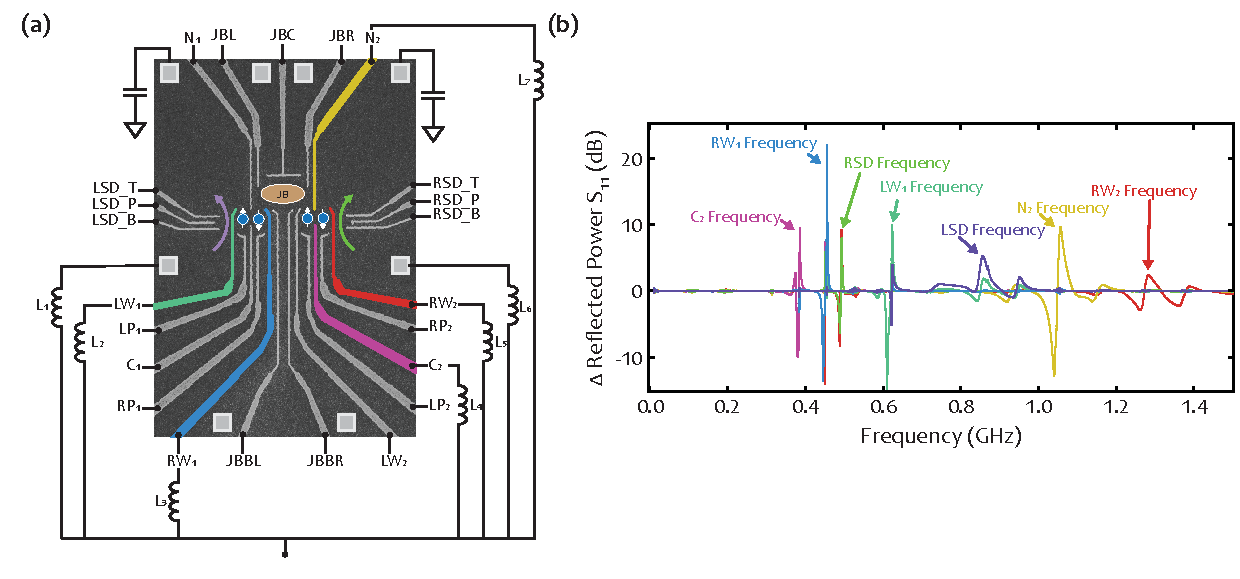
\includegraphics[width=\linewidth]{multifreq}
  \caption[Frequency multiplexed readout of a five-dot device]
  {\label{fig:multifreq}(a) False color SEM of a Five Dot device, identical to the one used in Sec.~\ref{sec:5dot}. A number of resonators are bonded to several gates
  including both charge sensors and dispersive gate sensors. (b) The frequency response of the multiplex chip when the voltage on each gate is changed. Distinct frequencies
  are observed for each gate on the sample.}
\end{figure}

An alternative to using a proximal charge sensor is to use the confining gates themselves as sensors~\cite{PhysRevLett.110.046805}, wherein the quantum capacitance
of the system is measured. The polarizability of a quantum dot is given by:
\begin{equation}
  C_Q = - \diffp[2]{E}{{V_{g}}} = -(\alpha \varepsilon)^2 \diffp[2]{E}{\varepsilon}
  \label{eq:cq}
\end{equation}
where $\alpha$ is the lever arm and $\varepsilon$ is the tilt, as shown in Fig.~\ref{fig:dqd} and defined in Sec.~\ref{sec:qd}. As we can see from the above equation
the quantum capacitance is proportional to the band curvature, which allows us not only to detect charge transitions but also the spin state (since the triplet state has no
curvature at 0 tilt), and hybridization. The latter effect may be used to detect the parity state of a Majorana zero mode coupled to a proximal
quantum dot~\cite{PhysRevB.95.235305}. As with readout via a charge sensor, by embedding a gate in a resonant circuit, we are able to quickly sense changes
in capacitance, with a sensitivity that is sufficient to perform single shot readout of spin states~\cite{fernando1,Nnano_dzurak}. A frequency multiplexed device
with 7 resonators is shown in Fig.~\ref{fig:multifreq}, combining both dispersive and charge-sensing modes of readout.

The potential for frequency multiplexing also allows us to imagine integrated methods of readout. While the idea of multi-channel qubit readout is certainly
not new, the design of equipment that are able to handle large numbers of channels simultaneously is as yet an open problem. In particular, once multiple
channels are multiplexed onto a single rf pair, the total power that must be transmitted for $n$ channels is:
\begin{equation}
  P_\sum(n) = P_0 + 10 \log_{10}(n)
\end{equation}
At the device level, this increases the isolation necessary between channels, as it is desirable to be able to select qubits to measure selectively. In addition,
crosstalk may drive rotations of neighbouring qubits, reducing the fidelity of control, which is particularly problematic for error correction schemes
where proximal ancilla qubits must be constantly read and corrected.

At this point, it is also worth covering noise in the readout circuit, as noise in the system is the limiting factor in readout time. Unfortunately, as alluded
to in earlier sections, the fragile nature of the quantum state requires us to use low probe powers in order to ensure our readout does not destroy the quantum
state. In quantum dots, we can generally place limits on the power of our probe signal $P_\textrm{probe}$ using similar thermal arguments to those used when discussing
bias, that is the power of the signal should be much less than the relevant energy scales of the system: $P_\textrm{probe} \ll \Delta E$. In the case of circuit-QED,
the requirements are even more strict, where operation in the single photon limit is necessary:
\begin{equation}
  P_\textrm{probe} \sim \frac{\hbar \omega^2}{2} \frac{Q_c}{Q_l^2}
\end{equation}
where $Q_c$ is the coupling-$Q$ and $Q_l$ is the loaded-$Q$ of the resonator. Unfortunately any quantum system will, at the very minimum, generate thermal noise and
vacuum fluctuations. The thermal noise power spectral density, that is the noise power per unit bandwidth, for a system is given
by~\cite{RevModPhys.82.1155}\footnote{Note that this form of noise power spectral density is given by a quantum theory of noise. In the limit
of large temperature ($\hbar\omega \ll k_BT$), using the approximation $\coth (x) \approx 1/x$ for small x, we recover the classical formula for noise power
spectral density: $S(\omega) = k_B T$.}:
\begin{equation}
  S(\omega) = \frac{\hbar \omega}{2}\coth\left(\frac{\hbar\omega}{2k_BT}\right)
\end{equation}
from which we can define an effective noise temperature of the system:
\begin{equation}
  T_\textrm{eff} = \frac{S(\omega)}{k_B}
\end{equation}
We can therefore define the maximum signal-to-noise ratio of a system, that is the signal-to-noise of an ideal receiver at the output of our qubit, for a measurement
bandwidth of \SI{1}{\hertz}:
\begin{equation}
  \textrm{SNR}_\textrm{max} = \frac{P_\textrm{probe}}{S(\omega)}
\end{equation}
In order to read a small signal, since any physical readout hardware will have a limited dynamic range and will itself add noise, additional amplification is necessary.
We must therefore account for the noise added by any given amplifier, with the total effective system temperature:
\begin{equation}
  T_\textrm{sys} = T_{0} + \frac{T_{1}}{G_1} + \frac{T_{2}}{G_1G_2} + \ldots \frac{T_{n}}{G_1G_2 \ldots G_{n}}
\end{equation}
where $T_{0}$ is the noise temperature at the output of the qubit, and will include $T_\textrm{eff}$, the thermal noise of the qubit and any noise present on the
probe signal, and $T_k,G_k$ are the noise temperature and gain of each stage of amplification or attenuation in the chain. For a HEMT amplifier commonly used in
spin qubit experiments, a gain on the order of \SI{30}{\decibel} is common, with a noise temperature of $\sim \SI{3}{\kelvin}$\footnote{For example the CITLF3 amplifier
from Cosmic Microtech: \url{https://www.cosmicmicrowavetechnology.com/citlf3}}, such that the system noise temperature after the first stage of amplification
is $T_\textrm{sys} \approx \SI{3000}{\kelvin}$. As long as the noise temperature of subsequent amplifier has $T_n \ll \SI{3000}{\kelvin}$, the first stage amplifier
will set the effective system temperature. As this temperature is well in the classical limit, we can define the system signal-to-noise ratio,
for a bandwidth of \SI{1}{\hertz}, as:
\begin{equation}
  \textrm{SNR}_\textrm{sys} = \frac{P_\textrm{probe}}{k_B T_\textrm{sys}}
  \label{eq:r_snr}
\end{equation}

The choice of first stage amplifier is therefore critical in designing a readout chain. The use of frequency multiplexing reduces the scaling of power and high-bandwidth
lines to \SI{4}{\kelvin}, as shown in Table~\ref{tab:arch}, however it creates additional constraints. Namely we must balance the \SI{1}{\decibel} compression point and
the noise temperature of the amplifier to minimize the effective system temperature while maximizing the allowed probe power and the number of simultaneous channels that
may be read. In particular for quantum limited amplifiers such as Josephson parametric amplifiers and or traveling-wave parametric amplifiers~\cite{Macklin307}
where the dynamic range is limited, designs which specifically take into account the bandwidth and power requirements for multi-channel readout are required. In addition
to this, the isolation of the amplification chain from the qubits must be considered. An attenuator can be considered an element with gain $G_k < 1$, and a temperature
set by the stage it is on, such that any attenuation between qubit and the first stage amplifier can lead to a large increase in the effective signal temperature. For this
reason, on spin or Majorana based systems, there is generally no isolation up to the first stage amplifier, however for circuit-QED type experiments, or those that require
the use of parametric amplifiers, isolators with minimal losses must be used, significantly increasing the footprint of the readout chain. For this reason, in
chapter~\ref{sec:hall}, the use of the quantum Hall effect to form miniaturized isolators is explored.

\begin{figure}
  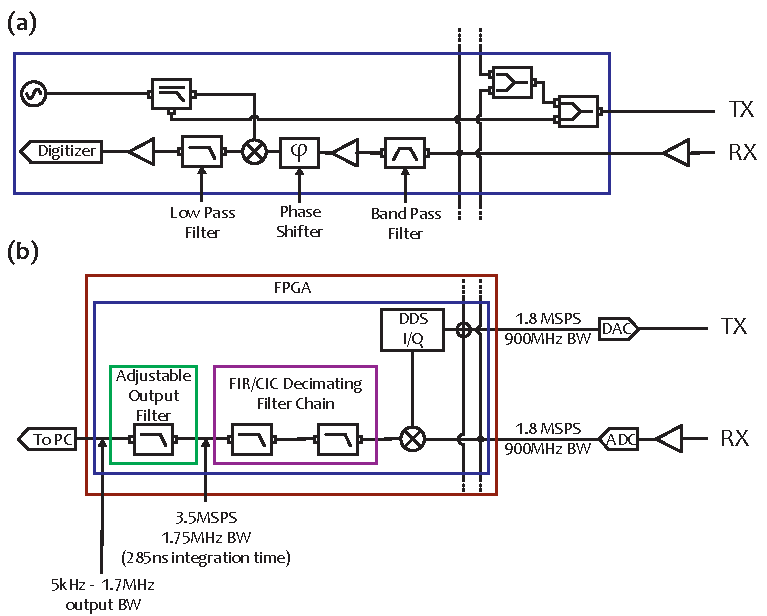
\includegraphics[width=0.8\linewidth]{Readout}
  \caption[Comparison of analog and digital multichannel readout]
  {\label{fig:multiread}(a) Schematic of an analog homodyne multichannel readout setup. Elements contained within the blue block must be repeated for each channel.
  A high-isolation band-pass filter is required per channel due to large non-linearities in the mixer. The use of a heterodyne receiver (not shown) allows phase
  sensitive detection, however requires a second analog signal generator. (b) The equivalent digital multichannel readout setup. Again, repeated elements are contained
  in the blue box, however in this case, all repeated elements are digital, hence require no additional hardware. Bandwidths for components used in our lab are shown.}
\end{figure}

Finally, we briefly touch on the topic of readout hardware at room temperature. The use of multiple simultaneous frequencies for readout creates several challenges
for a typical analog homodyne detection architecture, due to the higher-order non-linearity and the inherent unscalability of analog signal generators and low-bandwidth
digitizers. A schematic of a typical analog readout chain is shown in Fig.~\ref{fig:multiread} (a). Due to the non-linearities present in the analog mixer, signals must be
band-pass filtered and boosted prior to mixing to achieve optimal signal-to-noise. For the homodyne setup shown, an analog phase shifter is required, and does not allow
phase information to be extracted. A second analog signal source may be added prior to the mixer to allow for heterodyne (I/Q) demodulation, however this significantly
increases the resource requirements of the circuit. Therefore even with frequency multiplexing near the device, the scalability of an analog readout setup is still
linear in the number of qubits. An equivalent digital circuit is shown in Fig.~\ref{fig:multiread} (b). For such a readout chain, all repeated elements are in digital logic,
hence, up to the resource limits of the FPGA, no additional hardware is required to increase the channel count. Above around 32 channels, an alternative approach becomes
necessary, which I flag in Sec.~\ref{sec:gooseberry}, however I will not present results here.

Having introduced the general structure of an architecture for a semiconductor based quantum computer, the remainder of this chapter deals with the practical implementation
of some architectures, which progressively reduce the power dissipated and resource requirements at each stage of the architecture, at the expense of flexibility.
Section~\ref{sec:primelines} proposes an architecture for a quantum computer that reduces the need for high-bandwidth wiring to low temperature, covers the distribution of pulses
at the qubit interface and introduces low power cryogenic switches to accomplish that goal. Section~\ref{sec:gooseberry} proposes an architecture that utilizes CryoCMOS to drastically
reduce the wiring requirements for a large scale quantum computer, and creates a platform for scalable control of large numbers of qubits.

\clearpage
\section{Cryogenic Control Architecture for Large-Scale Quantum Computing}
\label{sec:primelines}
\import{chap2/}{arch}

\clearpage
\section[A CryoCMOS Based Control Architecture for Scaling Quantum Computers]{A CryoCMOS Based Control Architecture for Scaling Quantum Computers}
\label{sec:gooseberry}
\begingroup
  \addtocounter{footnote}{-1}
  \renewcommand\thefootnote{}
  \footnotetext{This section is based on unpublished work, and will include the following authors: S. J. Pauka, K. Das, R. Kalra, A. Moini, Y. Yang, J. D. Watson, G. C. Gardner, S. Fallahi, M. J. Manfra, D. J. Reilly}
\endgroup

In Sec.~\ref{sec:control} and Sec.~\ref{sec:readout}, the requirements for control and readout of semiconductor qubits were discussed, including a discussion
of where power is unavoidably dissipated in the system. These power requirements were summarized in Table~\ref{tab:arch}. While experiments involving a single qubit, or even a few qubits, have been able to sidestep the issues associated with such power dissipation at the various temperature stages of the cryostat, moving past as few as 20 qubits quickly becomes impractical. This can be seen if one considers the typical cooling power of these stages. Using the BlueFors LD-400 system~\cite{bluefors}
as an example of a typical dilution refrigerator, and using a Cryomech PT420 pulse tube cryocooler~\cite{cryomech} for cooling
to \SI{4}{\kelvin}, we find a cooling power of $\sim \SI{100}{\micro\watt}$ at the mK stage and \SI{2}{\watt} at the \SI{4}{\kelvin} stage when operating at
temperatures of \SI{40}{\mk} and \SI{4.2}{\kelvin} on the mK and \SI{4}{\kelvin} stages respectively. Under similar assumptions to those laid out in Sec.~\ref{sec:control} we find a maximum capacity of only 20 control lines at the \SI{4}{\kelvin} stage and 100 control lines at the mK stage. Using the Prime-Lines architecture presented in Sec.~\ref{sec:primelines}, the cooling requirements at \SI{4}{\kelvin} are reduced. However, solutions for scaling control lines at mK remain open.

In this section, we propose a CryoCMOS based architecture to reduce the wiring requirements and power dissipation at the lowest stages of a dilution refrigerator. This architecture
fixes the number of static lines required to define a semiconductor-based qubit to three, by providing a mechanism by which static voltages may be "locked" onto the gate, and for
reducing the growth of power consumption at the mK stage of the dilution refrigerator by generating fast control pulses near the qubit interface. In this way, the power
consumption is reduced from the dissipation through filters on the coaxial lines, to a $CV^2f$ dissipation set by the length of the interconnect between the qubit and the pulse
generator. This approach is validated using a quantum-dot based qubit device formed on a \ce{GaAs}/\ce{(Al,Ga)As} heterostructure, which is used to characterize the operation of
our CryoCMOS architecture at a temperature of $\sim \SI{40}{\milli\kelvin}$. Bringing together the ideas of Sec.~\ref{sec:primelines} with our CryoCMOS architecture, we demonstrate
a path for scaling to 100's of qubits within the power budget of commercially available dilution refrigerators.

\subsection{The CryoCMOS Architecture}
\label{sec:gbarch}

Our proposed CryoCMOS architecture is shown in Fig.~\ref{fig:gbarch} (a). Here, a CryoCMOS chip (orange) acts as an interface to the qubit chip (green), multiplexing a small number
of low-frequency dc lines from room temperature to the qubit chip. Control is provided by a microcontroller at the 4K stage of the dilution refrigerator. Readout multiplexing is provided by a series of resonators~\cite{doi:10.1063/1.4868107} following standard techniques for rf-reflectometry~\cite{Reilly:2007ig,barthel2009rapid}. Our CryoCMOS chip implementing this architecture is shown in Fig.~\ref{fig:gbarch} (b). Bond pads around the outside of the chip are used to interface with the microcontroller at 4K, and with the qubit device. Each qubit gate contains a charge-lock fast-gate cell, a simplified schematic of which is given in Fig.~\ref{fig:gbarch} (c).

\begin{figure}
  \includegraphics[width=\linewidth]{GBArch_Fig1}
  \caption[Schematic of our proposed CryoCMOS architecture]
  {\label{fig:gbarch}(a) Schematic of our proposed CryoCMOS architecture for qubit control. A fast control multiplexing chip allows a qubit chip to be controlled by a small number of digital control lines running from a microcontroller placed at \SI{4}{\kelvin}. Analog voltages are generated at room temperature using a low-noise, high-resolution DAC, and are multiplexed by the chip. Qubit readout is multiplexed using frequency multiplexing~\cite{doi:10.1063/1.4868107}. (b) Micrograph of the fast control multiplexing device. The chip has dimensions $2.5\times2.5\si{\milli\meter}$. (c) Simplified circuit schematic of a single charge-lock fast-gate cell. One cell is connected to each gate of the qubit device. A description of the operation is given in the text. (d) Time trace showing the output waveform as $G_\textrm{FG}$ is switched. The voltage at the output cell is pulsed between $V_\textrm{P}$ and $V_\textrm{HOLD}$, with sample period $\tau$. (e) Block diagram of the control circuitry inside the CryoCMOS chip.  SPI is used for digital communication to a microcontroller at 4K, which allows waveforms to be loaded into memory and pulse generation to be controlled. A voltage controlled oscillator is used to generate a clock on-chip and controls the sample period $\tau$.}
\end{figure}

Static voltages are provided for gates via a mechanism termed charge locking. In this technique, a high-precision room temperature DAC is used to set a voltage $V_\textrm{HOLD,N}$ on a
gate, selected by closing the switch $G_\textrm{LOCK,N}$, shown in Fig.~\ref{fig:gbarch} (b). A capacitance $C_\Sigma$ is charged and the switch $G_\textrm{LOCK,N}$ is opened, leaving a voltage set on the gate. The total capacitance is set by the capacitance of the bond-wires and by parasitic capacitances on the gates of both the CryoCMOS device and the qubit device. Although similar schemes for locking charges on devices have been proposed in the literature~\cite{PhysRevApplied.9.054016,doi:10.1063/1.4932012}, they have suffered from gate voltage leakage rates of several mV per hour, limiting the applicability of such schemes for multiplexing large numbers of gates, as refresh times of several ms would be required.

Charge locking allows a large number of static gates on the qubit device to be operated from a minimal number of lines running from room temperature. However, the power or footprint required to bring down even thousands of dc lines is not prohibitive, nor is there a current limitation in connecting such a large number of lines to a qubit device. Instead, the principal limitation at present is the dissipation of power in high-bandwidth control lines. As given in Eq.~\ref{eq:phot}, reducing the population of thermal photons necessarily involves attenuation or filtering at the mK stage. Hence, to decrease power consumption at this stage, either qubits must be built to be resilient to thermal noise, allowing
the magnitude of the attenuation to be reduced, or signal routing and generation must occur at the mK stage, allowing a smaller number of coaxial lines to be used. Designing qubits
that are immune to noise is an ongoing area of research~\cite{PhysRevB.93.121410,PhysRevLett.121.177701,PhysRevB.97.155402}, however, these approaches trade off insensitivity for large amplitude control pulses. Even for Majorana qubits, the excitation of quasiparticles in a superconductor, which acts as an error mechanism in these qubits, places limits on a minimum amount of filtering that is necessary~\cite{PhysRevLett.106.167004}. It is, therefore, the second approach that we explore here, implementing a two-level
fast pulse generator on-chip.

Control pulses are generated on the CryoCMOS device using a method we term fast gating. A ground reference is set on the CryoCMOS chip, through the capacitor $C_\textrm{PULSE}$, referenced
either to the voltage $V_\textrm{LOW}$ or $V_\textrm{HIGH}$. To generate a control pulse on the charge-locked output voltage, the two switches controlled by $G_\textrm{FG,N}$ are rapidly pulsed,
pulling or pushing charges on the output gate, and causing a change in $V_\textrm{OUT,N}$. A sketch of this operating principle is shown in Fig.~\ref{fig:gbarch} (d), where the magnitude of the pulse $\Delta V_\textrm{PULSE} = V_\textrm{P} - V_\textrm{HOLD}$ is given by:
\begin{equation}
  \Delta V_\textrm{PULSE} = \frac{C_\textrm{PULSE}}{C_\textrm{P} + C_\textrm{PULSE}} (V_\textrm{HIGH} - V_\textrm{LOW})
\end{equation}
Crucially, by placing the CryoCMOS chip in close proximity to the qubit chip, such that parasitic capacitance $C_p$ is minimized, the power dissipated for a given pulse can be minimized.
Assuming the system can be described by a lumped element model, valid in the limit that the qubit is near the CryoCMOS chip, the power dissipated in the system is given by:
\begin{equation}
  P_\textrm{diss} = \frac{C_\textrm{PULSE} + C_\textrm{P}}{C_\textrm{PULSE}C_\textrm{P}} \left(V_\textrm{HIGH} - V_\textrm{LOW}\right)^2 f
  \label{eq:diss}
\end{equation}
where $f$ is the average rate of pulses at the device.

A block diagram of the control logic for the CryoCMOS architecture is given in Fig.~\ref{fig:gbarch} (e). An on-chip waveform memory stores up to 256-time steps of a waveform. An on-chip voltage controlled oscillator is used to drive waveforms, which can be enabled by a small finite state machine. The waveform sampling period can be changed in two ways,
the first is by varying the value of TRIM, which changes the clock speed in 6 exponential steps between roughly \SI{6}{\mega\hertz} and \SI{140}{\mega\hertz}, the second is using
the clock divider FDIV, which may be varied in linear steps from 2 to 256. The waveform sampling period $\tau$ can, therefore, be changed between roughly \SI{23}{\kilo\hertz} at
(TRIM = 1, FDIV = 255), and \SI{70}{\mega\hertz} at (TRIM = 6, FDIV = 2).

\subsection{Benchmarking the CryoCMOS chip}

\begin{figure}
  \includegraphics[width=\linewidth]{GBArch_Fig2}
  \caption[Testbench for the CryoCMOS architecture]
  {\label{fig:gbtb}(a) Image of the test setup used to benchmark our CryoCMOS chip. A quantum-dot based qubit chip is shown in green, containing a total of 6 five-quantum-dot devices, similar to those introduced in Sec.~\ref{sec:5dot}. For the purposes of this test, a single double quantum dot is bonded to the CryoCMOS chip, while a second double quantum dot is bonded directly to static control lines. The CryoCMOS chip is shown in orange, while readout multiplexing chips are shown in purple. (b) False color micrograph of the double quantum dot structure. Orange colored gates are controlled directly by a room-temperature DAC, while blue colored gates are controlled by the CryoCMOS chip. Gates are labeled in black. (c) Coulomb blockade through a single quantum dot formed using the CryoCMOS chip to control all quantum dot gates (LW, LP, C, RP, RW), with C sufficiently low that a double quantum dot does not form.}
\end{figure}

The performance of the charge locking system for static control is benchmarked using a quantum-dot based qubit device, shown in Fig.~\ref{fig:gbtb} (a).
The qubit device (green) is a comprised of six 5-dot devices, similar to the ones presented in Sec~\ref{sec:5dot}, although for the purposes of this test, only a single double-quantum dot is used in the top right of the chip. A scanning electron micrograph of the device is shown in Fig.~\ref{fig:gbtb} (b).
Five of the confining gates, labeled LW, LP, C, RP, and RW, are connected to the CryoCMOS chip with bond-wires, while the remaining gates, SDT, SDP, SDC, and N, are connected directly to the room temperature DAC. It is, therefore, possible to benchmark the CryoCMOS chip with only a single charge-locked gate, passing current through O1 to O2 and measuring a quantum point contact (QPC) formed with the gates SDT and LW, or to benchmark all 5 gates used to define a double quantum dot. As an initial validation of the concept, a single quantum dot is formed using all five CryoCMOS controlled gates and is shown in Fig.~\ref{fig:gbtb} (c). To take this plot, a static voltage of \SI{-0.5}{\volt} is set on gates LP, C, and RP. For each column of data, a voltage is
set and held on gate LW by toggling the switch $G_\textrm{LOCK,LW}$, following which $G_\textrm{LOCK,RW}$ is closed and the voltage $V_\textrm{HOLD}$ on the right wall is swept.

\begin{figure}
  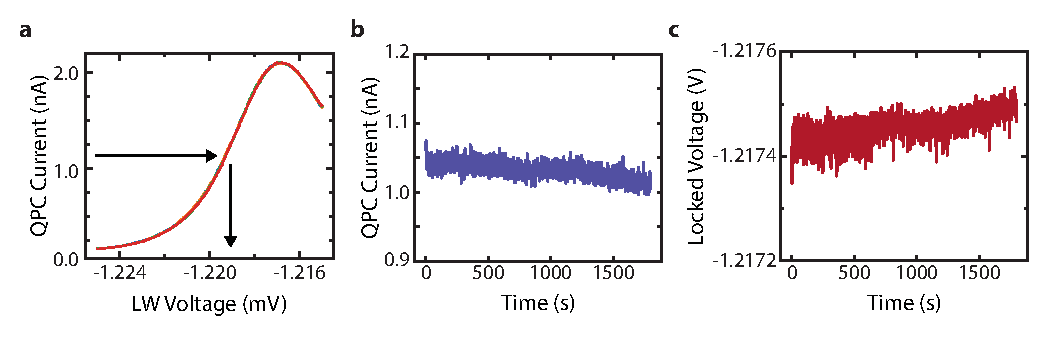
\includegraphics[width=\linewidth]{GBArch_Fig3}
  \caption[Voltage calibration procedure and hold time]
  {\label{fig:gbvc}Calibration procedure to extract gate voltage. (a) Calibration curves are taken while sweeping LW with the $G_\textrm{LOCK}$ switch closed, such that the gate is directly driven. Here four traces are overlaid, validating the stability of the device. Black arrows show how a current through the QPC is converted into a gate voltage. (b) Current through a QPC formed using the gate SDT and LW, once a voltage has been locked on the CryoCMOS controlled gate LW. (c) Extracted value for the CryoCMOS locked voltage on LW, after running the trace in (a) through the calibration curve in (b).}
\end{figure}

To properly characterize the leakage rate of voltages held using the CryoCMOS switches, we form a QPC between the gates SDT and LW. The voltage on SDT is set to
a constant value, and the value of $V_\textrm{HOLD}$ is swept with $G_\textrm{LOCK,LW}$ closed, while a current between ohmics O1 and O2 is measured. This measurement is
repeated several times to ensure the device is stable and is shown in Fig.~\ref{fig:gbvc} (a). Following this, the voltage is tuned to the steepest point of the QPC pinch-off
curve, around \SI{1.1}{\nano\ampere} in Fig.~\ref{fig:gbvc} (a), and held over a 30 minute period, yielding a slow drift in current as shown in Fig.~\ref{fig:gbvc} (b).
Combining Fig.~\ref{fig:gbvc} (a) and Fig.~\ref{fig:gbvc} (b), a value for the voltage locked on the gate is extracted in Fig.~\ref{fig:gbvc} (c). Noise in the measurement
is caused by low-frequency charge noise present in the 2DEG~\cite{PhysRevApplied.9.034008}.

\begin{figure}
  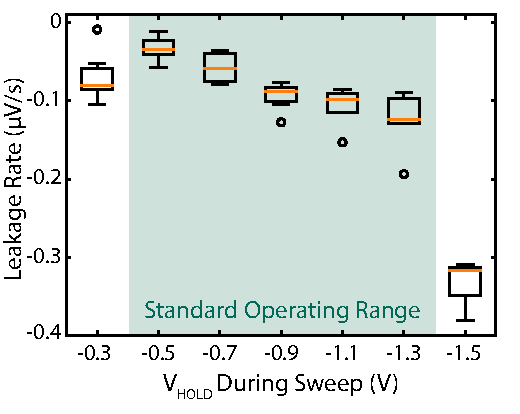
\includegraphics[width=0.5\linewidth]{GBArch_Fig4}
  \caption[Leakage rate of charge locking]
  {\label{fig:gblr}Leakage rate of charge locking as the value of $V_\textrm{HOLD}$ is varied during the hold. For each datapoint the QPC is tuned to its most sensitive point,
  which occurs around $V_\textrm{LW} = \SI{-0.83}{\volt}$, and the gate is held for 1 hour. At either extreme of the operating range (\SIrange{-0.5}{-1.3}{\volt}), the leakage
  rate is found to be unstable.}
\end{figure}

A full characterization of the leakage rate is performed following the procedure laid out in Fig.~\ref{fig:gbvc}, with a hold time of \SI{1}{\hour}, for a period of \SI{65}{\hour}. Between subsequent sweeps, the QPC is retuned such that sweeps begin at the most sensitive starting point. The optimal value of $V_\textrm{LW}$ was found to vary between \SIrange{-0.838}{-0.840}{\volt} over the course of measurements, due to low frequency drift in the device~\cite{PhysRevApplied.9.034008}. The resting value of $V_\textrm{HOLD}$ during the hold sequence is varied to account for increased leakage when the voltage difference across the switch $G_\textrm{LOCK,LW}$ is changed. The results of this sweep are shown in Fig.~\ref{fig:gblr}. Across the operating range of \SIrange{-0.5}{-1.3}{\volt} the average leakage rate was found to be \SI{-81.7}{\nano\volt\per\second} or \SI{-294}{\micro\volt\per\hour}. Despite the voltage difference across the switch $G_\textrm{LOCK,LW}$ changing from a value less than $V_\textrm{LOCK,LW}$ to a value greater than $V_\textrm{LOCK,LW}$, the leakage is uniformly found to be negative, suggesting it is occurring via the wells of the transistor which are biased to \SI{-1.8}{\volt}. To our knowledge, this is the lowest leakage rate for a charge locked device reported in the literature.

\begin{figure}
  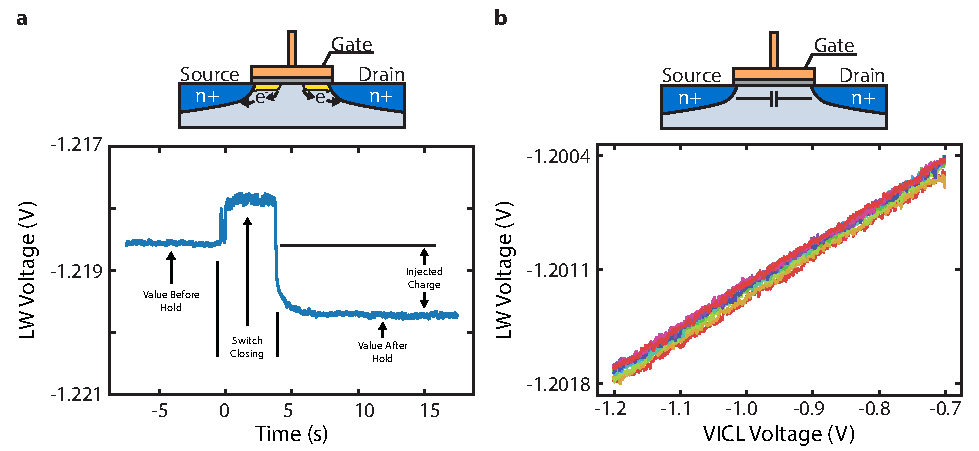
\includegraphics[width=0.9\linewidth]{GBArch_Fig5}
  \caption[Static corrections to hold voltage]
  {\label{fig:gbcorr} (a) Effect of charge injection when opening the switch $G_\textrm{LOCK}$. The charges that form the channel are pushed onto the gate, leading to an offset voltage before and after the switch is opened. This effect can equivalently be understood as a stray capacitance between the gate and drain leads of a transistor. (b) Stray capacitance across the switch, leading to a change in the voltage held on a gate as the disconnected value of $V_\textrm{HOLD}$ is swept.}
\end{figure}

Finally, we highlight two sources of parasitic capacitance that must be compensated for in a real device. The first of these is the effect of charge injection~\cite{1052859}, caused by the movement of electrons that form the conductive channel in the MOSFET into the source and drain leads, shown schematically in the top panel of Fig.~\ref{fig:gbcorr} (a). When either of these leads is not driven, as is the case when a voltage is held on a gate, an offset in the voltage results after the switch is opened. This effect may be modeled as a simple gate-drain capacitance $C_\textrm{GD}$, with a correction for the quantum capacitance built into this value to account for the density of states in the channel, as given in Eq.~\ref{eq:cq}. The offset in gate voltage caused by charge injection $\Delta V_\textrm{CI}$ is then given by:
\begin{equation}
  \Delta V_\textrm{CI} = \frac{C_\textrm{GD}}{C_\textrm{GD} + C_\textrm{P} + C_\textrm{PULSE}} \SI{1.8}{\volt}
\end{equation}
where \SI{1.8}{\volt} is the operating voltage of the MOSFETs, and $C_\textrm{P}$ and $C_\textrm{PULSE}$ are the capacitances holding the voltage of the gate, as shown in Fig.~\ref{fig:gbarch} (c). The effect of charge injection is shown in Fig.~\ref{fig:gbcorr} (a), and for a single gate is found to take a constant offset of \SI{-1.12}{\milli\volt} which can be compensated prior to the locking of a charge on a gate. We also highlight that this effect may be compensated in the design stage of the CryoCMOS through techniques known in the literature~\cite{45719}.

The second source of parasitic capacitance that must be compensated is the source-drain capacitance $C_\textrm{SD}$ across the charge locking switch, as shown schematically in the top panel of Fig.~\ref{fig:gbcorr} (b). This capacitance leads to a small change $\Delta V_\textrm{SD}$ in the charge locked voltage, given by:
\begin{equation}
  \Delta V_\textrm{SD} = \frac{C_\textrm{SD}}{C_\textrm{SD} + C_\textrm{P} + C_\textrm{PULSE}} (V_\textrm{HOLD} - V_\textrm{GATE})
\end{equation}
For the LW gate, a change of $\Delta V_\textrm{SD} = \SI[per-mode=symbol]{2.8}{\milli\volt\per\volt}$ is observed, as shown in Fig.~\ref{fig:gbcorr} (b). Again, this effect may be trivially compensated prior to the locking of a charge on a gate by selecting a fixed value of $V_\textrm{HOLD}$ during the operation of the qubit device.

\subsection{Fast Gating}
Finally, we move on to describe the generation of fast pulses at the level of the device. Having described the method used to generate pulses in Sec.~\ref{sec:gbarch}, we utilize a quantum dot formed against the LW gate with three directly controlled gates, SDT, SDP, and SDB. In this way, we can again characterize the behavior of our CryoCMOS architecture using only a single directly controlled gate. To first extract the expected behavior of fast gating, the value of $V_\textrm{LOW}$ is set to \SI{-0.4}{\volt} and $V_\textrm{HIGH}$ is set to \SI{-0.396}{\volt}, and a 1D trace is taken and shown in Fig.~\ref{fig:gbfg} (a), sweeping $V_\textrm{SDP}$, with $C_\textrm{FG,LW}$ first set to $V_\textrm{LOW}$ in blue, followed by $V_\textrm{HIGH}$ in red. Following this, a fixed frequency square waveform is loaded into the waveform memory and run, and the 1D sweep is retaken. The results are shown in green and show a square wave pattern that switches rapidly between the trace taken against $V_\textrm{LOW}$ and taken against $V_\textrm{HIGH}$.

\begin{figure}
  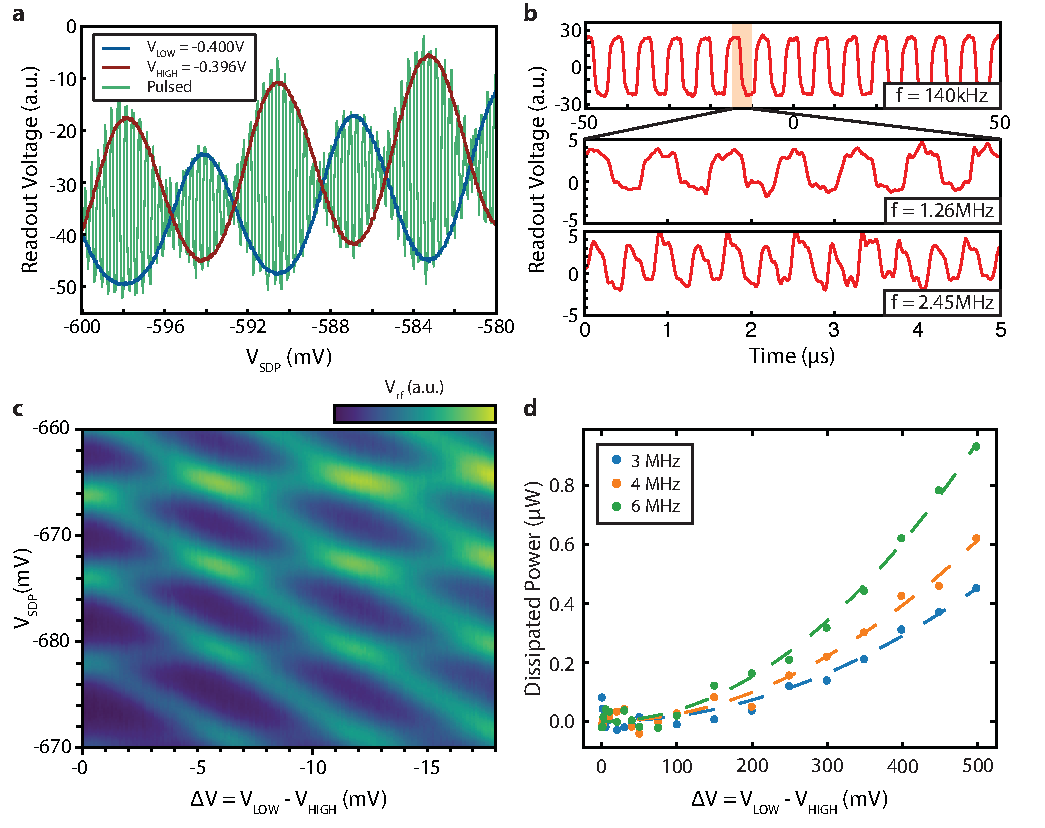
\includegraphics[width=0.9\linewidth]{GBArch_Fig6}
  \caption[Characterization of fast gating]
  {\label{fig:gbfg} (a) Demonstration of fast gating. $V_\textrm{LOW}$ is set to \SI{-0.4}{\volt} and $V_\textrm{HIGH}$ is set to \SI{-0.396}{\volt}. Before fast gating is enabled, $G_\textrm{FG,LW}$ is set to $V_\textrm{LOW}$ (blue trace) and $V_\textrm{SDP}$ is swept on the room temperature DAC, followed by the same trace taken with $G_\textrm{FG,LW}$ set to $V_\textrm{HIGH}$. Fast gating is then enabled while $V_\textrm{SDP}$ is swept (green), showing a trace that pulses between the two slow traces. (b) Demonstration of the tunability of frequency. The top trace shows a square wave at \SI{140}{\kilo\hertz}, the middle trace at \SI{1.26}{\mega\hertz} and the bottom trace at \SI{2.45}{\mega\hertz}. (c) Tunability of the
  pulse amplitude by sweeping $V_\textrm{HIGH} - V_\textrm{LOW}$. Here $V_\textrm{LOW}$ is held constant while $V_\textrm{HIGH}$ is varied, such that one set of coulomb peaks remains
  horizontal, while the other moves to more negative voltages. (d) Power dissipated at the mixing chamber as $V_\textrm{HIGH} - V_\textrm{LOW}$ is swept, due to $CV^2f$ dissipation. Dashed lines are parabolic fits to the data.}
\end{figure}

Having validated that pulse generation works, we now show that the frequency and amplitude of the pulses may be varied. As described in Sec.~\ref{sec:gbarch}, the sample may be modified in several ways, including by changing the tuning the VCO, through the clock divider and by appropriate choice of the waveform. In Fig.~\ref{fig:gbfg}, we show the variation of the frequency of a square wave from \SI{140}{\kilo\hertz}, up to \SI{2.45}{\mega\hertz} through alteration of the clock divider and waveform. Measurements above this frequency are limited by the readout setup; however, we note the potential for operation up to a sample period of \SI{140}{\mega\hertz}.

Variation of the pulse amplitude is performed by changing the difference $\Delta V$ between the voltages $V_\textrm{HIGH}$ and $V_\textrm{LOW}$. In general, as gates that are not intended to be pulsed have voltages set in reference to $V_\textrm{LOW}$, this value will remain fixed, while $V_\textrm{HIGH}$ is varied. In Fig.~\ref{fig:gbfg} (c), the value of $V_\textrm{HIGH}$ is varied on the bottom axis while $V_\textrm{SDP}$ is swept. The pulse frequency is configured to be well above the bandwidth of the readout circuit, such that an averaged trace between $V_\textrm{HOLD}$ and $V_\textrm{P}$ is returned. As such, as $\Delta V$ is increased from zero, each coulomb peak splits into two, with one remaining at the same value of $V_\textrm{SDP}$, and the other decreasing towards more negative values of $V_\textrm{SDP}$ as $V_\textrm{HIGH}$ is increased to more positive values.

Combining these effects, we can extract the power dissipation of the entire circuit. The cooling power of the mixing chamber of the dilution refrigerator is first calibrated using a known resistance. Then, as various circuits on the CryoCMOS chip are enabled, the extra heating of the device is calculated. The static power dissipation for the circuit is extracted to be $\sim \SI{0.1}{\micro\watt}$ based on the current drawn on the power rails. Upon enabling the clock, an additional \SI{9}{\micro\watt} of static power dissipation and \SI[per-mode=symbol]{2.5}{\micro\watt\per\mega\hertz} of dynamic power is dissipated by the clock generation circuitry. We note that although this is a significant portion of the power budget at mK, this dissipation is static at a fixed frequency, as this clock is shared by all gates. To extract the heating due to pulses applied to gates, pulses at a known frequency are applied and $\Delta V$ is swept. As the total length of routing and bond-wires is on the order of millimeters, a lumped element model is sufficient to calculate dissipation, such that the aggregate dissipated power is given by Eq.~\ref{eq:diss}. From this, a total capacitance to ground of \SI{0.6}{\pico\farad} is extracted. The power per gate controlled, assuming a pulse amplitude of \SI{1}{\milli\volt} at \SI{10}{\mega\hertz} is therefore only \SI{6}{\pico\watt}, on top of a static power dissipation of \SI{34}{\micro\watt}, well within the cooling power of a typical dilution refrigerator.

\subsection{Conclusion}
We have proposed a CryoCMOS based architecture for scaling qubit devices up to the hundreds without a large increase in power dissipated at the mK stage of a dilution refrigerator. By placing a CryoCMOS pulse generator close to the qubit chip, the power dissipation per channel may be lowered to 10's of pico-watts. Using our CryoCMOS chip, we are also able to lock static control voltages on gates with a leakage rate of \SI{-294}{\micro\volt\per\hour}, the lowest value reported in the literature, allowing the number of static control lines to be reduced to a minimum of three. For large scale quantum machines, we anticipate that some form of cryogenic pulse generation, such as the one presented here, will be crucial to allow large numbers of qubits to be controlled without unacceptable heat dissipation in high-bandwidth control lines.

\subsubsection{Acknowledgments}
This research was supported by the Microsoft Corporation and the Australian Research Council Centre of Excellence for Engineered Quantum Systems (EQuS, CE170100009). The authors acknowledge the facilities as well as the scientific and technical assistance of the Research \& Prototype Foundry Core Research Facility at the University of Sydney, part of the Australian National Fabrication Facility
